%! Author = mr
%! Date = 3/27/2025

\section{Time Dilation from Vortex Dynamics}\label{sec:Part-1}
We consider an inviscid, irrotational superfluid æther with stable topological vortex knots. The Æther experiences absolute time $t_{\text{abs}}$, but local clocks experience slowed rates due to pressure gradients and knot energetics. The Vortex Æther Model posits that the rate at which time flows in the local frame (near the knot) depends on the internal angular frequency $\Omega_k$. In this section, we derive time dilation analogues inspired by the predictions of general relativity (GR), based solely on pressure and vorticity gradients in the fluid.

\begin{figure}[h!]
    \centering
    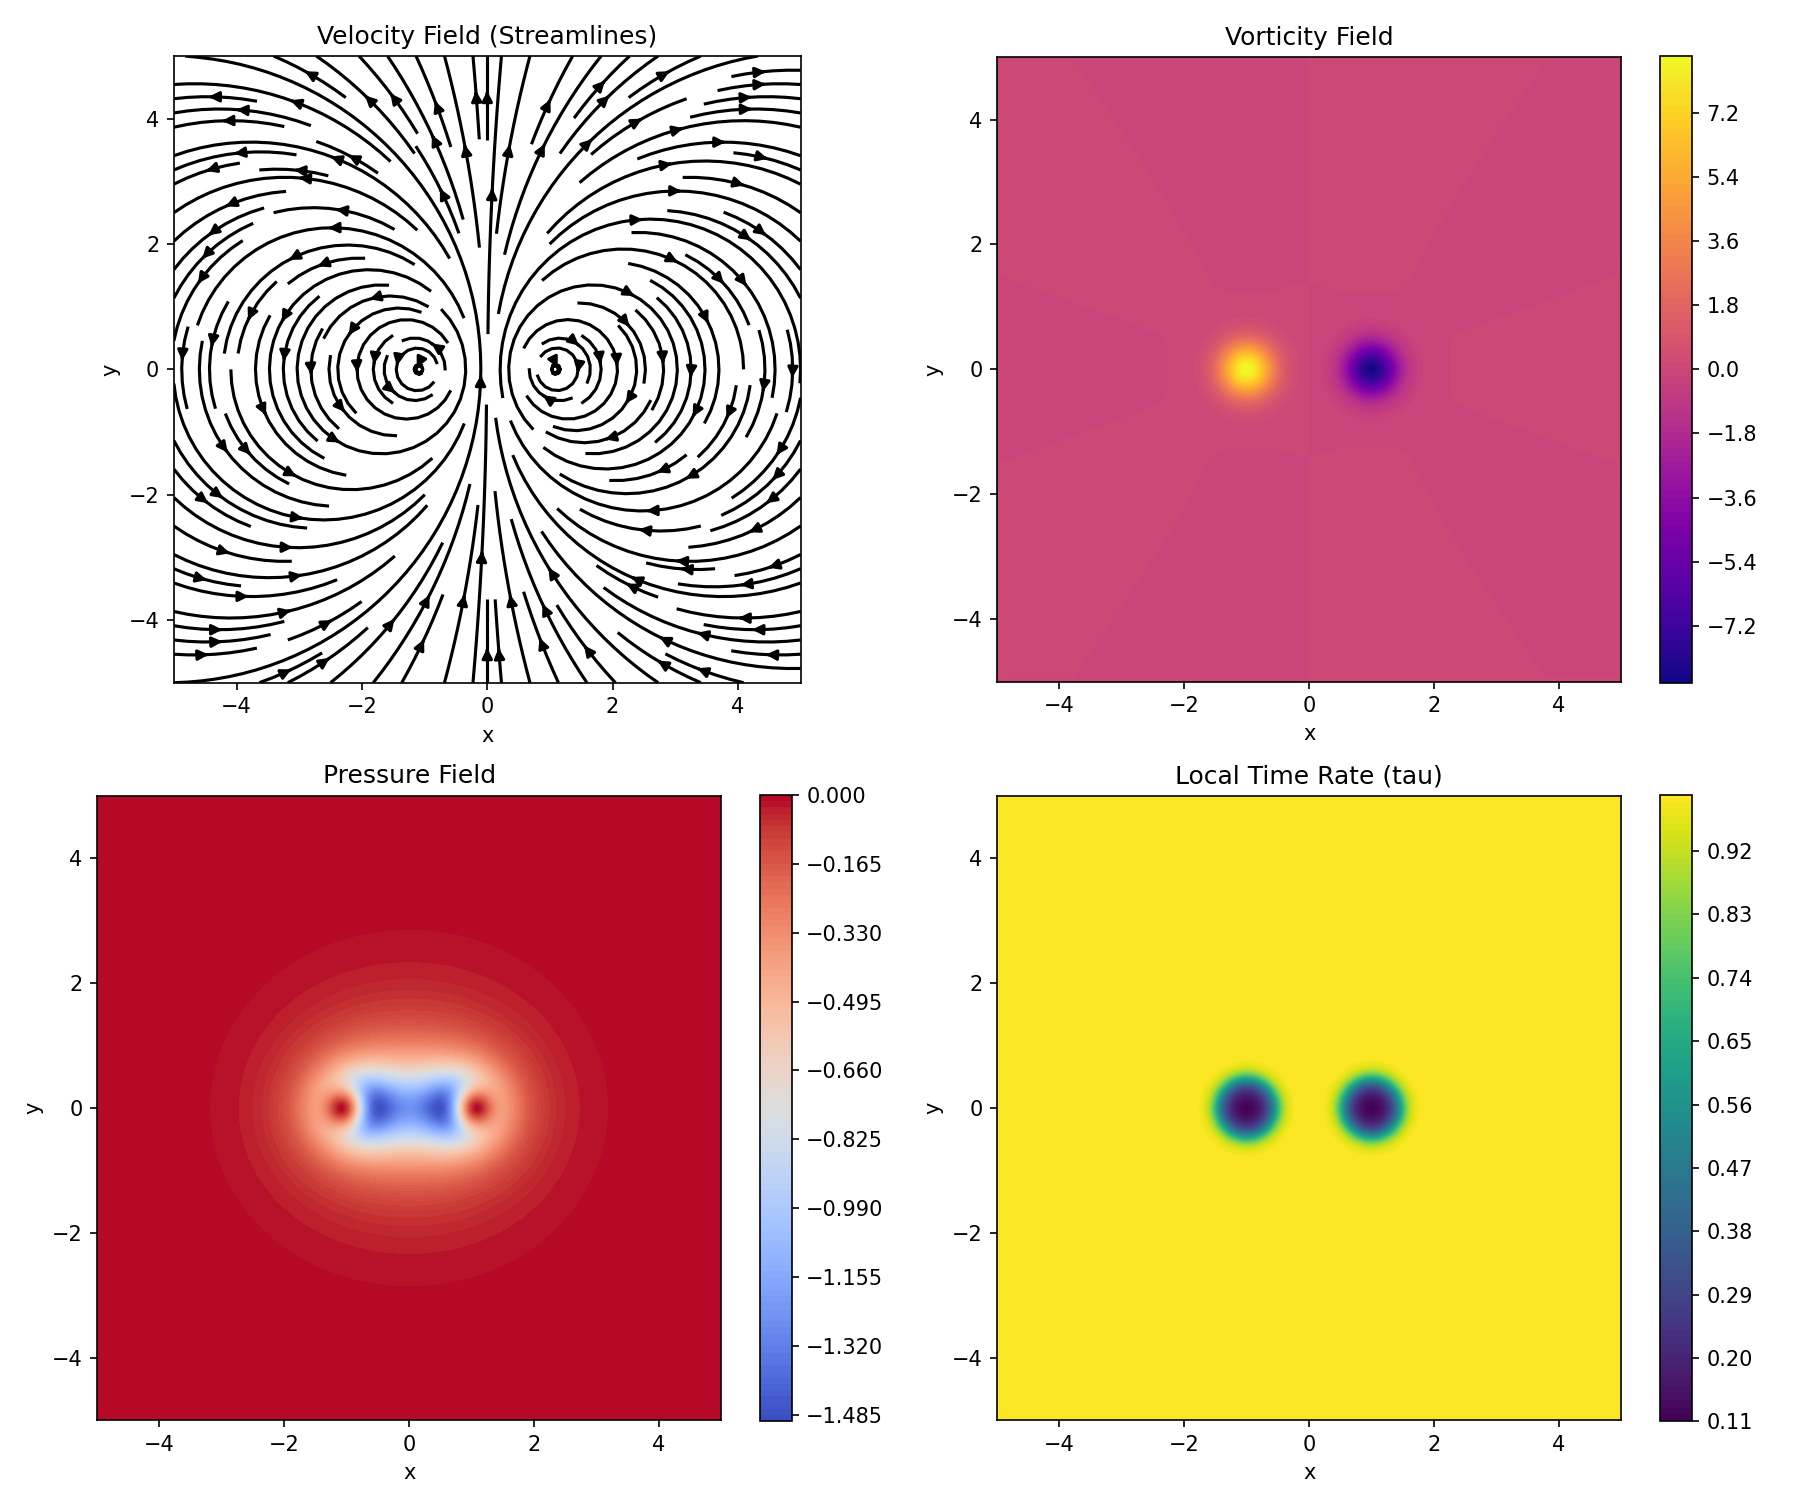
\includegraphics[width=0.85\textwidth]{export/streamlinesDiPole}
    \caption{Velocity streamlines, vorticity, pressure, and local time rate $\tau$ for a simulated vortex pair. The pressure minimum and time slow-down clearly align with the regions of high vorticity. This directly illustrates the æther model's central claim: time dilation follows from vortex energetics and pressure depletion.}
    \label{fig:vortexfields}
\end{figure}

\subsection{Bernoulli \& Rotational Flow}
In high-vorticity zones, Bernoulli's principle implies a local drop in pressure:
\begin{equation}
    \frac{1}{2} \rho_\text{æ} v^2 + p = p_0 \quad \Rightarrow \quad p = p_0 - \frac{1}{2} \rho_\text{æ} v^2
\end{equation}
Assuming the local frequency of a clock is proportional to Æther pressure:
\begin{equation}
    f_{\text{local}} = f_0 \left(1 - \frac{\rho_\text{æ} v^2}{2p_0} \right)
\end{equation}
Thus, the time dilation becomes:
\begin{equation}
    \frac{t_{\text{local}}}{t_0} = \left(1 - \frac{\rho_\text{æ} v^2}{2p_0} \right)^{-1}
\end{equation}
For circular vortex motion with $v = \Omega r$:
\begin{equation}
    \frac{t_{\text{local}}}{t_0} \approx 1 + \frac{\rho_\text{æ} \Omega^2 r^2}{2p_0}
\end{equation}
This is analogous to special relativistic dilation if $\rho_\text{æ}/p_0 \sim 1/c^2$.

\begin{figure}[h!]
    \centering
    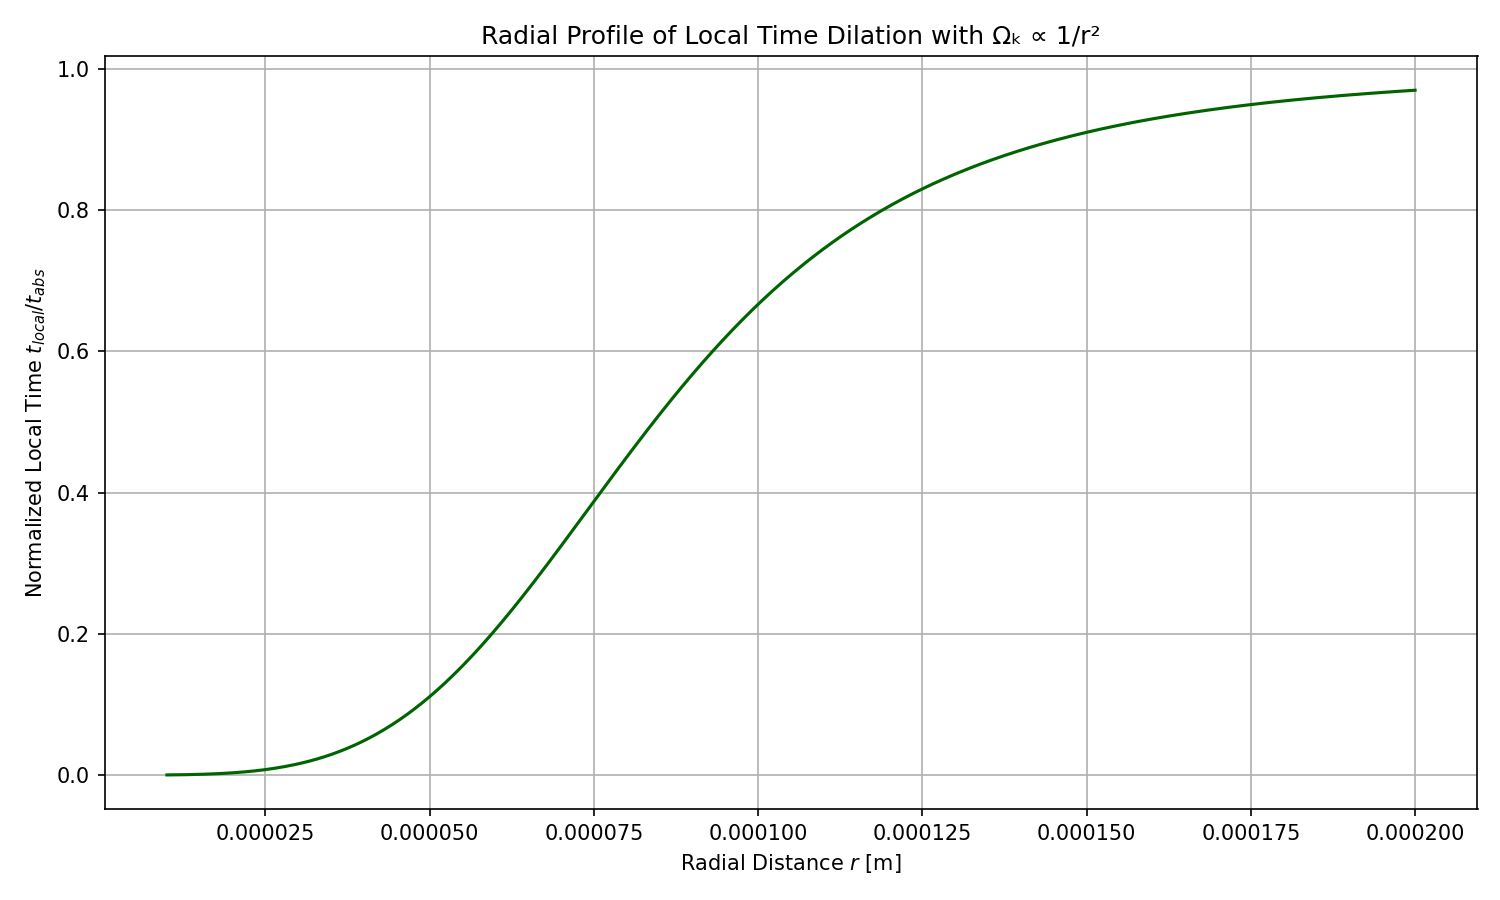
\includegraphics[width=0.8\textwidth]{export/RadialProfileOfLocalTimeDilation_Radial_LocalTime_Dilation}
    \caption{Radial profile of normalized local time $t_{\text{local}} / t_{\text{abs}}$ as a function of distance $r$ from the vortex core, assuming $\Omega_k \propto 1/r^2$. Time slows significantly near the vortex center and recovers to background values with distance.}
    \label{fig:radial_time_profile}
\end{figure}

\subsection{Heuristic Knot-Based Time Modulation}
Topological vortex knots possess internal rotation. Let $\Omega_k$ be their average angular velocity. We postulate a heuristic time modulation law:
\begin{equation}
    \label{eq:heuristic}
    \frac{t_{\text{local}}}{t_{\text{abs}}} = \left(1 + \alpha \Omega_k^2 \right)^{-1}
\end{equation}
where $\alpha$ is a coupling constant related to the Æther's compressibility or inertia. For small $\Omega_k$, we expand:
\begin{equation}
    \frac{t_{\text{local}}}{t_{\text{abs}}} \approx 1 - \alpha \Omega_k^2 + \mathcal{O}(\Omega_k^4)
\end{equation}
This expression parallels the Lorentz factor for low velocities:
\[
    \frac{t_{\text{moving}}}{t_{\text{rest}}} \approx 1 - \frac{v^2}{2c^2}
\]

\begin{figure}[h!]
    \centering
    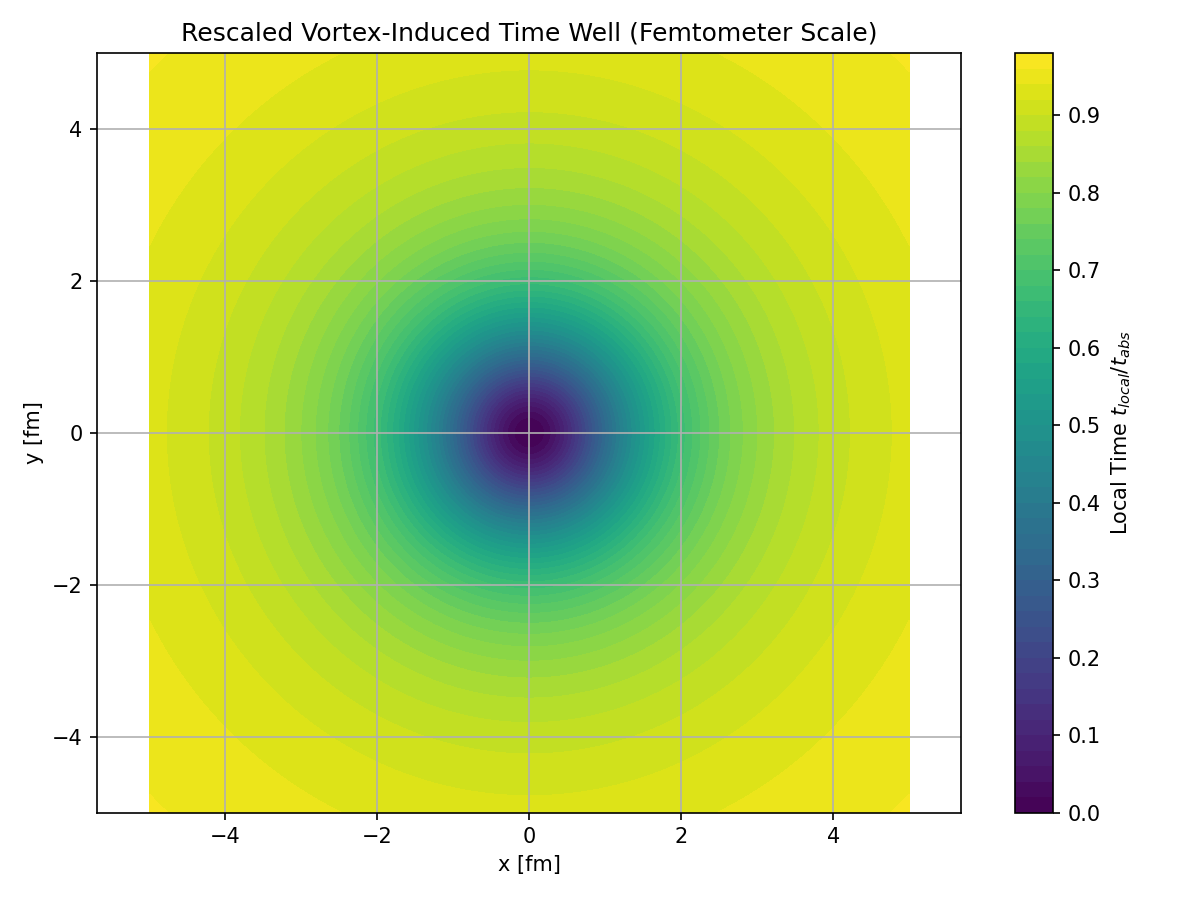
\includegraphics[width=0.8\textwidth]{export/RadialProfileOfLocalTimeDilation_Vortex-Induced_Time_Well}
    \caption{Schematic of a vortex-induced time well in the æther. Local time $t_{\text{local}} / t_{\text{abs}}$ is shown as a color gradient in 2D space. The central vortex region exhibits the most time slowing due to high $\Omega_k$, forming a well-like structure.}
    \label{fig:vortex_time_well}
\end{figure}


\subsection{Energetic Interpretation: Rotational Inertia}
The above heuristic can be grounded in the rotational energy of vortex knots. Let $I$ be the effective moment of inertia of a knot, then the energy stored is:
\begin{equation}
    E_\text{rot} = \frac{1}{2} I \Omega_k^2
\end{equation}
Assuming the time dilation arises from this stored energy modifying local information rates:
\begin{equation}
    \frac{t_{\text{local}}}{t_{\text{abs}}} = \left(1 + \alpha I \Omega_k^2 \right)^{-1}
\end{equation}
This model provides a bridge between fluid rotation and gravitational-like time shifts, replacing the need for spacetime curvature with internal knot energetics. It suggests that time flow slows where circulation is topologically conserved.

\begin{equation}
    \boxed{
        t_{\text{local}} = \frac{t_{\text{abs}}}{1 + \alpha I \Omega_k^2}
    }
\end{equation}
This boxed result summarizes the time modulation law driven by rotational inertia.

\subsection{Conclusion and Experimental Outlook}
The Vortex Æther Model replaces spacetime curvature with conserved vorticity in a 3D fluid. Time dilation arises from localized pressure depletion and kinetic energy storage within vortex knots, offering a classical, topological reinterpretation of relativistic effects. In this formulation, time slows in regions of high vorticity due to pressure depletion, aligning with relativistic predictions \cite{fedi2017gravity, simula2020gravitational, winterberg1990maxwell}. Future work includes simulations of vortex clocks and tests using BECs, helium II, or electrohydrodynamic lifters.


